\documentclass[a4paper, 10pt]{article}
\usepackage[a4paper, margin=2cm]{geometry}
\usepackage[utf8]{inputenc}
\usepackage[T1]{fontenc}
\usepackage{graphicx}
\usepackage{amsmath}
\usepackage{listings}
\usepackage{xcolor}
\usepackage{hyperref}
\usepackage{caption}
\usepackage{subcaption}
\usepackage{booktabs}
\usepackage{array}
\usepackage{etoolbox}
\usepackage{setspace} % line spacing control
\usepackage{parskip}  % No paragraph indentation
\usepackage{ragged2e} % Better left alignment

\hypersetup{
    colorlinks=true,
    linkcolor=black,
    filecolor=magenta,      
    urlcolor=blue,
    pdftitle={Business-IT Alignment Dynamics},
    pdfpagemode=FullScreen,
}


\usepackage{minted}
\usemintedstyle{xcode} 
\usepackage{inconsolata} 

\setminted{
  frame=single,
  framesep=10pt,
  fontsize=\small,        
  linenos=false,  
  bgcolor=white,       
  breaklines=true,
  breakanywhere=true,
}

\title{Business-IT Alignment Dynamics: A Chaotic Systems Approach}
\author{Alessandro Aquilini}
\date{\today}

\begin{document}
\setstretch{1.1} % 1.1x line spacing
\raggedright     % clean left alignmen

\maketitle

\begin{abstract}
	Lorem Ipsum
	% This report investigates the dynamics of Business-IT alignment through a discrete-time chaotic model. The proposed equation captures how environmental pressures, IT department efficacy, and organizational adaptability interact to create alignment or misalignment patterns. Through numerical simulations and bifurcation analysis, we identify conditions leading to stable alignment, oscillations, and chaotic behavior.
\end{abstract}

\tableofcontents

\section{Introduction}
% \subsection{Objective}
% The project aims to model Business-IT alignment dynamics using a discrete-time equation that exhibits chaotic behavior under certain parameter conditions. The primary goals are:
%
% \begin{itemize}
% 	\item Develop a mathematical model of alignment evolution
% 	\item Implement interactive simulations in Python
% 	\item Analyze stability and chaotic regimes
% 	\item Provide visual tools for parameter exploration
% \end{itemize}
%
% \subsection{Key Findings}
% \begin{itemize}
% 	\item The system shows three characteristic behaviors: convergence, oscillations, and chaos
% 	\item IT department efficacy ($a$) and system rigidity ($h$) have non-linear effects
% 	\item Organizational flexibility ($s$) determines adaptation sharpness
% 	\item Bifurcation diagrams reveal parameter regions of chaotic behavior
% \end{itemize}

\section{User Requirements}
\subsection{Target Audience}
This interactive notebook is designed for anyone interested in Business-IT alignment dynamics.
It also serves as template for modeling other complex dynamics using discrete time equations in the form: $x_{t+1} = x_t + \Delta(t, \text{*args})$. The user just needs to apply a few minor customization to the code.

\subsection{Getting Started}
\subsubsection{Installation}
\begin{enumerate}
	\item Clone the repository:
	\begin{lstlisting}[language=bash]
git clone https://github.com/Kinshale/pii.git
cd pii
    \end{lstlisting}

	\item Install required packages:
	\begin{lstlisting}[language=bash]
pip install numpy matplotlib ipywidgets
    \end{lstlisting}
\end{enumerate}

\subsubsection{Running the Notebook}
Choose your preferred environment:
\begin{itemize}
	\item \textbf{Local Jupyter}: Launch Jupyter Notebook and open \texttt{pii.ipynb}
	\item \textbf{VS Code}: Open the notebook with Jupyter extension
	\item \textbf{Google Colab}:
	      \begin{enumerate}
		      \item Visit \url{https://colab.research.google.com}
		      \item Select "GitHub" tab and paste the notebook URL
		      \item Or open the cloned one
	      \end{enumerate}
\end{itemize}

For optimal experience:
\begin{itemize}
	\item Start with default parameters to observe baseline behavior
	\item Modify one parameter at a time to understand its effect
	\item Use the bifurcation tool to identify chaotic parameter regions
\end{itemize}

\section{Model Description}
\subsection{Core Equation}
The alignment dynamics are governed by:

\begin{equation}
	x_{t + 1} = x_t + A(x_t) - B(x_t)C(x_t)
\end{equation}

Where:
\begin{itemize}
	\item $x_t$: Percentage of dissatisfied users (misalignment proxy)
	\item $A(x_t)$: Environmental pressure effect
	\item $B(x_t)$: IT department efficacy
	\item $C(x_t)$: Organizational adaptability
\end{itemize}

\subsection{Component Functions}
\begin{align}
	A(x_t) & = d(1 - x_t)                                                                     \\
	B(x_t) & = \frac{a x_t (1 - x_t)^g}{1 + a h x_t}                                          \\
	C(x_t) & = \frac{1}{1 + z^s} \quad \text{where} \quad z = \frac{r (1 - x_t)}{x_t (1 - r)}
\end{align}

\subsection{Parameter Definitions}
\begin{table}[h]
	\centering
	\caption{Model Parameters and Ranges}
	\begin{tabular}{llll}
		\toprule
		\textbf{Parameter} & \textbf{Description}       & \textbf{Range} & \textbf{Default} \\
		\midrule
		$x_0$              & Initial misalignment       & [0.01, 0.99]   & 0.3              \\
		$d$                & Environmental dynamicity   & [0.01, 5]      & 0.5              \\
		$a$                & IT department efficacy     & [0.1, 10]      & 2                \\
		$h$                & IT system rigidity         & [0.1, 5]       & 1                \\
		$g$                & IT investment propensity   & [0.1, 5]       & 1                \\
		$r$                & Action threshold           & [0.01, 0.99]   & 0.3              \\
		$s$                & Organizational flexibility & [1, 10]        & 3                \\
		\bottomrule
	\end{tabular}
\end{table}

\subsection{Interpretation}
Let's take a deeper look at our equation:

\begin{equation}
	x_{t + 1} = x_t + \underbrace{A(x_t)}_{\text{Environmental Pressure}} - \underbrace{B(x_t)C(x_t)}_{\text{Recovery Mechanism}}
\end{equation}

\begin{description}
	\item[$x_t$ \textendash\ Alignment] Measures the percentage of dissatisfied users at time $t$:
		\begin{itemize}
			\item $0 \rightarrow$ Complete satisfaction (perfect alignment)
			\item $1 \rightarrow$ Utter dissatisfaction (total misalignment)
		\end{itemize}

	\item[$A(x_t)$ \textendash\ Environmental Pressure:] Increases misalignment due to external factors, representing how competitive environments and technological changes increase dissatisfaction.

	\item[$B(x_t) \cdot C(x_t)$ \textendash\ Recovery Mechanism:] Reduces misalignment through:
		\begin{itemize}
			\item $B(x_t)$: IT department's effectiveness.
			\item $C(x_t)$: Organization's adaptability.
		\end{itemize}
\end{description}

\subsection{Parameter Analysis}
Full interactive simulation available at: \url{https://www.desmos.com/calculator/n55bwehjlp}

\subsubsection{Environmental Pressure Function}
\begin{equation}
	A(x_t) = d(1 - x_t)
\end{equation}

Forms a line passing through $(1, 0)$ with slope $-d$.
\begin{itemize}
	\item \textbf{$d$ (dynamicity)}: Fast changing industries (e.g., a tech startup) have a competition/innovation that rapidly renders old IT systems obsolete.
	\item \textbf{$1 - x_t$}: As misalignment grows, environmental pressure has less "room" to worsen things.
\end{itemize}

\begin{figure}[h]
	\centering
	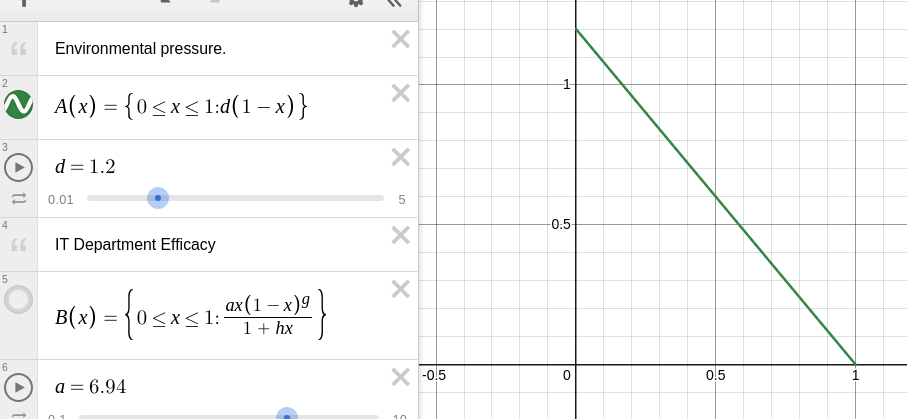
\includegraphics[width=0.8\textwidth]{../images/desmos/A(x)-desmos.png}
	\caption{Environmental pressure function for varying $d$ values}
\end{figure}

\subsubsection{IT Department Efficacy}
\begin{equation}
	B(x_t) = \frac{a x_t (1 - x_t)^g}{1 + a h x_t}
\end{equation}

This looks like a function that peaks at some $x_a$ and then tapers off.

\begin{itemize}
	\item \textbf{a (IT efficacy)}: an higher a can more effectively reduce misalignment.
	\item \textbf{x (current misalignment)}: the more misalignment exists, the more opportunity/pressure there is for IT to act.
	\item \textbf{$(1 - x_t)^g$ (Diminishing Returns)}: as satisfaction improves, the IT department's impact diminishes.
	      \begin{itemize}
		      \item I haven't understood g.
	      \end{itemize}
	\item \textbf{$1 + ahx_t$ (Saturation)}: even if IT is highly capable (a >> 1), inflexible systems (h >> 1) limit its efficacy.
\end{itemize}

\begin{figure}[h]
	\centering
	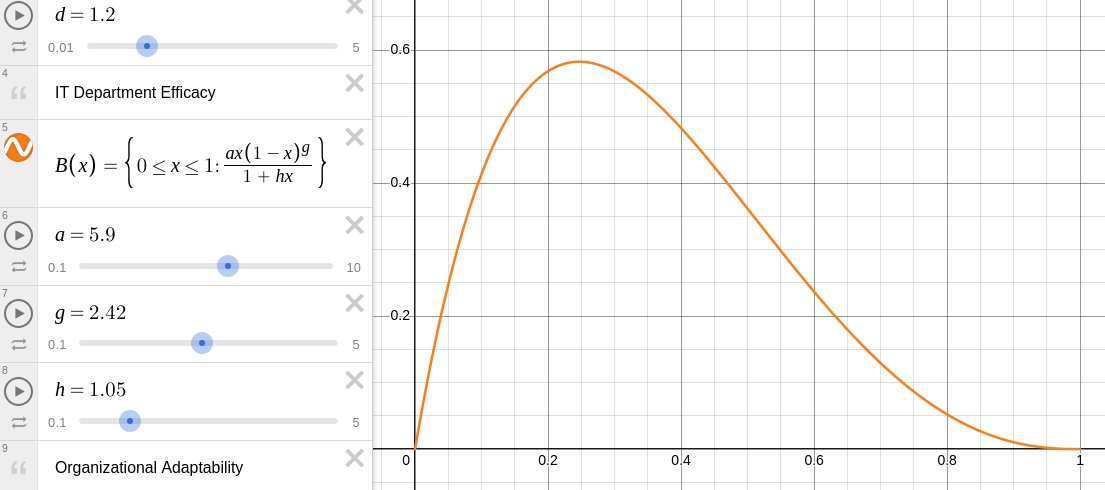
\includegraphics[width=0.8\textwidth]{../images/desmos/B(x)-desmos.png}
	\caption{IT efficacy function showing the effect of parameters $a$, $h$, and $g$}
\end{figure}

\subsubsection{Organizational Adaptability}
\begin{equation}
	C(x_t) = \frac{1}{1 + z^s} \quad \text{where} \quad z = \frac{r (1 - x_t)}{x_t (1 - r)}
\end{equation}

This is a \textbf{sigmoid} function in disguise. Sigmoids are exploited for modeling "threshold behaviors".

\begin{itemize}
	\item \textbf{r (activation threshold)}: below r, the organization resists to change ($C(x) \rightarrow 0$). But when misalignment crosses a certain threshold adaptability kicks in.
	\item \textbf{s (flexibility)}: higher s make the sigmoid steeper (sharper transition from resistance to adaptation).
\end{itemize}

\begin{figure}[h]
	\centering
	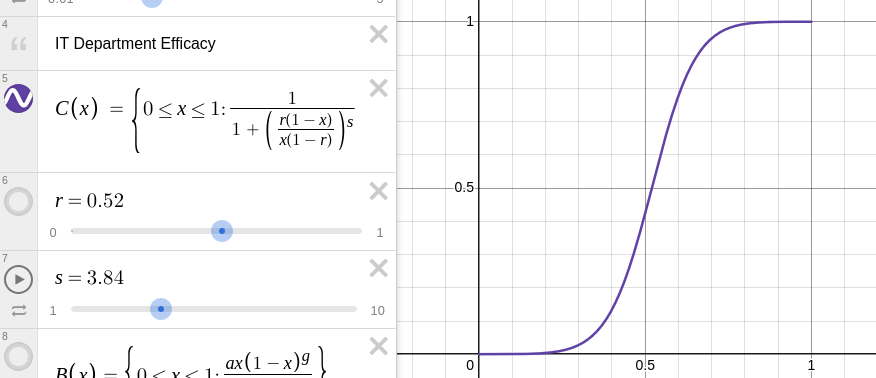
\includegraphics[width=0.8\textwidth]{../images/desmos/C(x)-desmos.png}
	\caption{Organizational adaptability function demonstrating threshold behavior}
\end{figure}


\section{Implementation}
\subsection{Technological Stack}
\begin{itemize}
	\item Python 3.10.12 (managed via Conda)
	\item Jupyter Notebook for interactive exploration, with markdown explanations attached
	\item Core dependencies (Python Libraries)
	      \begin{itemize}
		      \item NumPy for numerical computations
		      \item Matplotlib for visualization graphs
		      \item ipywidgets for parameter sliders
	      \end{itemize}
\end{itemize}

\subsection{Key lines of code}
\subsubsection{Simulating the equation}
The equation is hardcoded:

\begin{minted}{python}
def A(x, d):
    return d * (1 - x)

def B(x, a, h, g):
    return (a * x * (1 - x) ** g) / (1 + a * h * x)

def C(x, r, s):
    if x == 0:  # Avoid division by zero
        return 0
    z = (r * (1 - x)) / (x * (1 - r))
    return 1 / (1 + z ** s)

def delta(x, d, a, h, g, r, s):
    return A(x, d) - B(x, a, h, g) * C(x, r, s)

def simulate(x0, d, a, h, g, r, s, steps=100):
    x = np.zeros(steps)
    x[0] = x0
    for t in range(steps - 1):
        x[t + 1] = np.clip(x[t] + delta(x[t], d, a, h, g, r, s), 0, 1)
\end{minted}

\subsubsection{Long term behavior}
Here is the key logic behing classifing the equation.

\begin{minted}{python}
x = simulate(x0, d, a, h, g, r, s, steps)

last_values = x[-10:]

if np.std(last_values) < 0.001:  # Stable state
final_val = np.mean(last_values)
if final_val < 0.1:
    return x, "ALIGNED"
elif final_val > 0.9:
    return x, "MISALIGNED"
else:
    return x, "PARTIAL_ALIGNMENT"
else:  # Dynamic state
if len(np.unique(np.round(last_values, 2))) > 3:
    return x, "CHAOTIC"
else:
    return x, "OSCILLATING"
\end{minted}

\subsubsection{Phase Portrait Analysis}
The phase space visualization algorithm:

\begin{minted}{python}
def phase_portrait(d, a, h, g, r, s, n_points=200):
    x = np.linspace(0, 1, n_points)
    dx = np.array([delta(xi, d, a, h, g, r, s) for xi in x])
    
    # Arrow placement logic
    arrow_indices = np.linspace(0, len(x)-1, 20, dtype=int)
    norm = Normalize(vmin=0, vmax=np.max(np.abs(dx)))
    
    for xi, dxi in zip(x[arrow_indices], dx[arrow_indices]):
        if dxi > 0:  # Right arrow
            plt.arrow(xi, 0, 0.02, 0, ...)
        elif dxi < 0:  # Left arrow
            plt.arrow(xi, 0, -0.02, 0, ...)
    
    plt.plot(x, dx, 'k-')  # Main curve
    plt.axhline(0, color='black', linestyle=':')  # Zero line
\end{minted}

\subsubsection{Bifurcation Analysis}
The chaotic regime detection algorithm:

\begin{minted}{python}
def bifurcation_analysis(param, p_min, p_max, fixed_params, n_points=500):
    param_values = np.linspace(p_min, p_max, n_points)
    n_transient = 200  # Skip initial transient
    n_samples = 100    # Points to plot per parameter
    
    for p in param_values:
        params = fixed_params.copy()
        params[param] = p
        
        x = 0.3  # Initial value
        # Burn-in phase
        for _ in range(n_transient):
            x = np.clip(x + delta(x, **params), 0, 1)
        
        # Sample stable points
        x_vals = []
        for _ in range(n_samples):
            x = np.clip(x + delta(x, **params), 0, 1)
            x_vals.append(x)
        
        plt.plot([p]*n_samples, x_vals, 'k.', markersize=0.5)
\end{minted}

\subsection{Numerical Considerations}
\begin{itemize}
	\item State clipping ensures $x_t \in [0,1]$ remains meaningful
	\item All floating-point operations use NumPy's float64 precision
	\item The bifurcation analysis skips 200 transient iterations to focus on long-term behavior
	\item Phase portrait arrows are normalized to avoid cluttering
\end{itemize}

\section{Results}
\subsection{Interactive Tools}
The notebook provides three powerful ways to explore alignment dynamics.

\subsubsection{Time Evolution Simulation}
The time evolution simulation displays how alignment changes over successive iterations.
You can tweak the initial condition ($x_0$), the number of iterations and all the parameters of the equation through the \textbf{sliders}.
The diagram will update in real-time.

\begin{figure}[h]
	\centering
	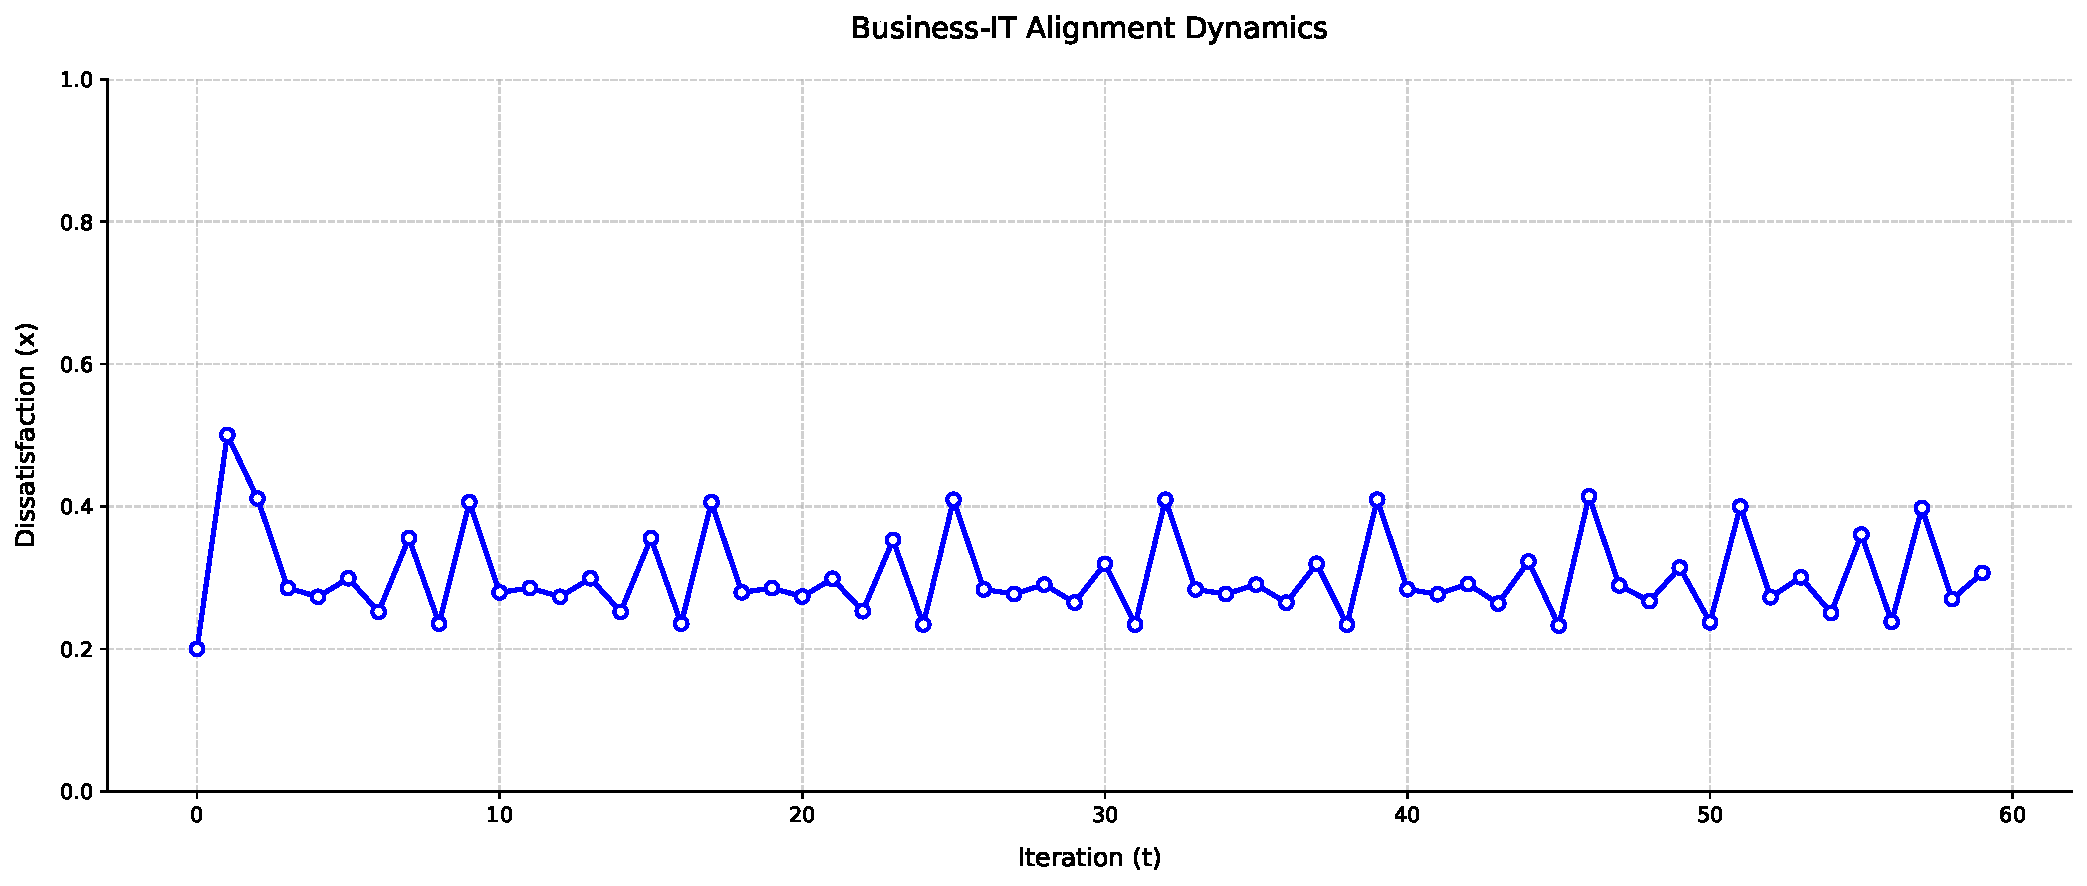
\includegraphics[width=1\textwidth]{../images/results/res-int-1.pdf}
	\caption{Time evolution showing chaotic behaviour ($d = 0.5$, $a = 6$, $h = 0.4$, $g = 2$, $r = 0.25$, $s = 5$)}
	\label{fig:time_sim}
\end{figure}

\subsubsection{Phase Portrait Analysis}
The phase portait examines the system's underlying dynamics through multiple visual cues. Arrow directions indicate whether misalignment tends to increase or decrease at each state point, while a color gradient represents the rate of change intensity.

\textbf{Note:} Stable equilibrium points occur where the curve crosses zero with a negative slope - these represent self-correcting alignment levels.

\begin{figure}[h]
	\centering
	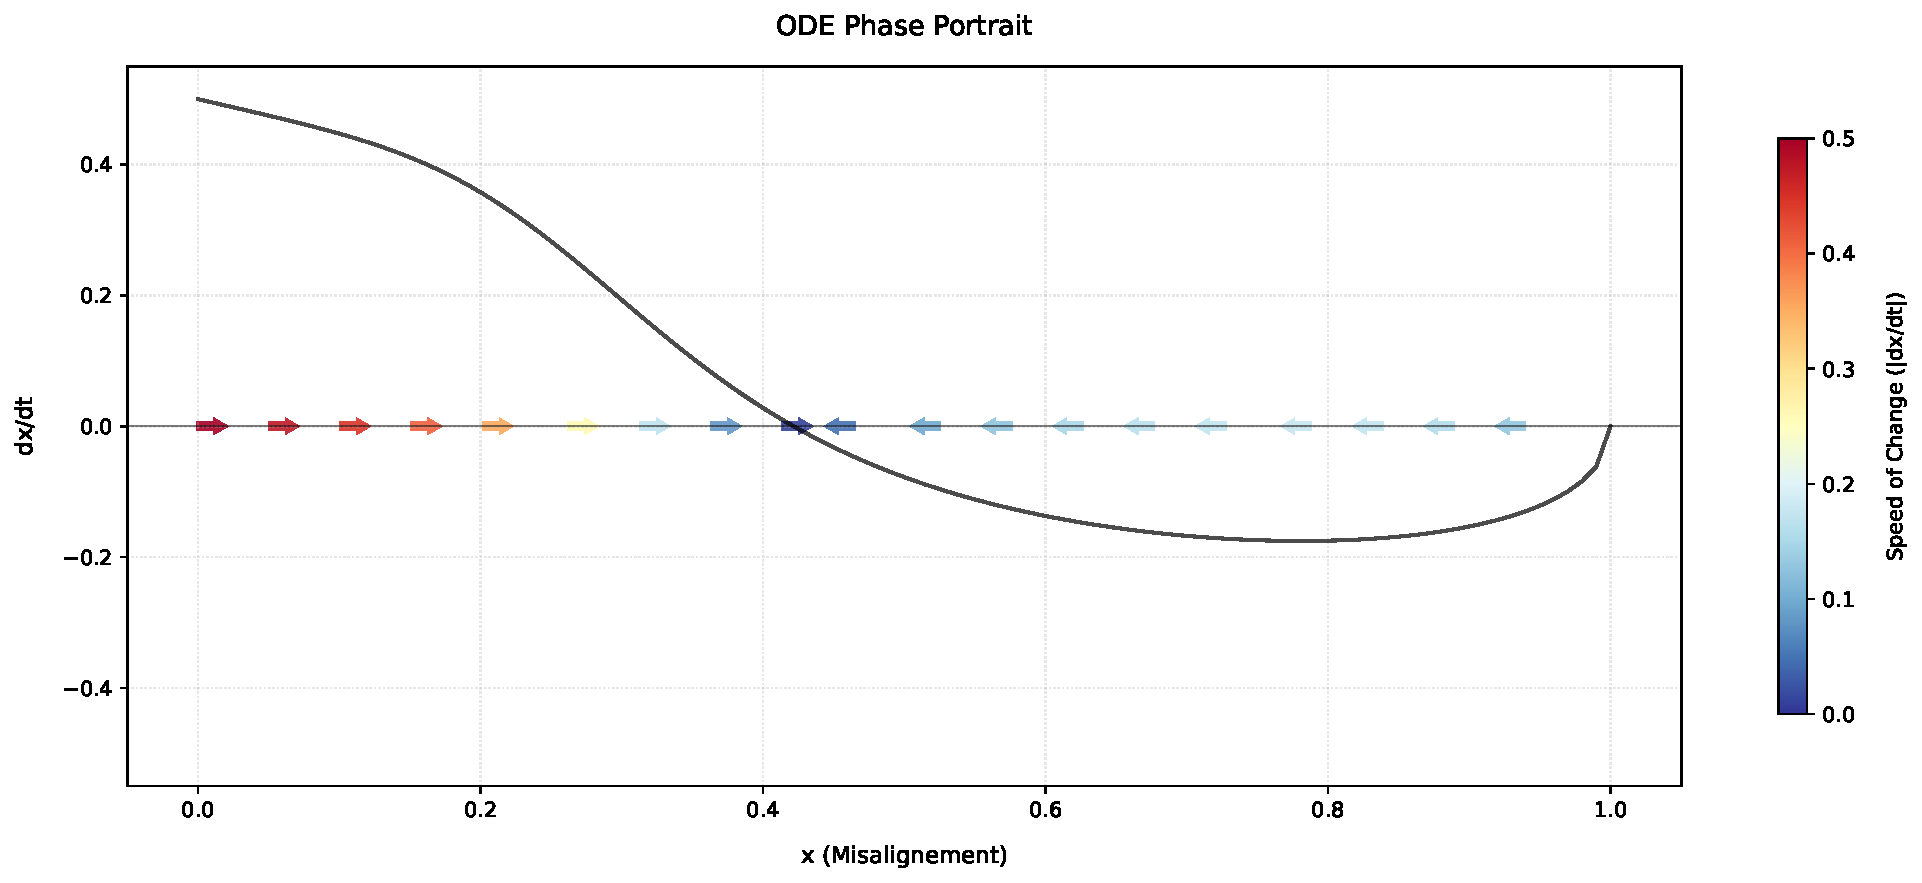
\includegraphics[width=1\textwidth]{../images/results/res-int-2.pdf}
	\caption{Phase portrait ($d = 0.5$, $a = 2$, $h = 1$, $g = 0.5$, $r = 0.3$, $s = 3$)}
	\label{fig:phase_portrait}
\end{figure}

\subsubsection{Bifurcation Diagram}
Users can select any parameter for the x-axis via a dropdown menu and focus on specific ranges of interest.
Adjust the sliders, and you may get the chacteristic period-doubling bifurcations and the emergance of chaotic behaviour.

\textbf{Pro tip:} Set $h$ (IT rigidity) to a low value for observing beatiful patterns.

\begin{figure}[h]
	\centering
	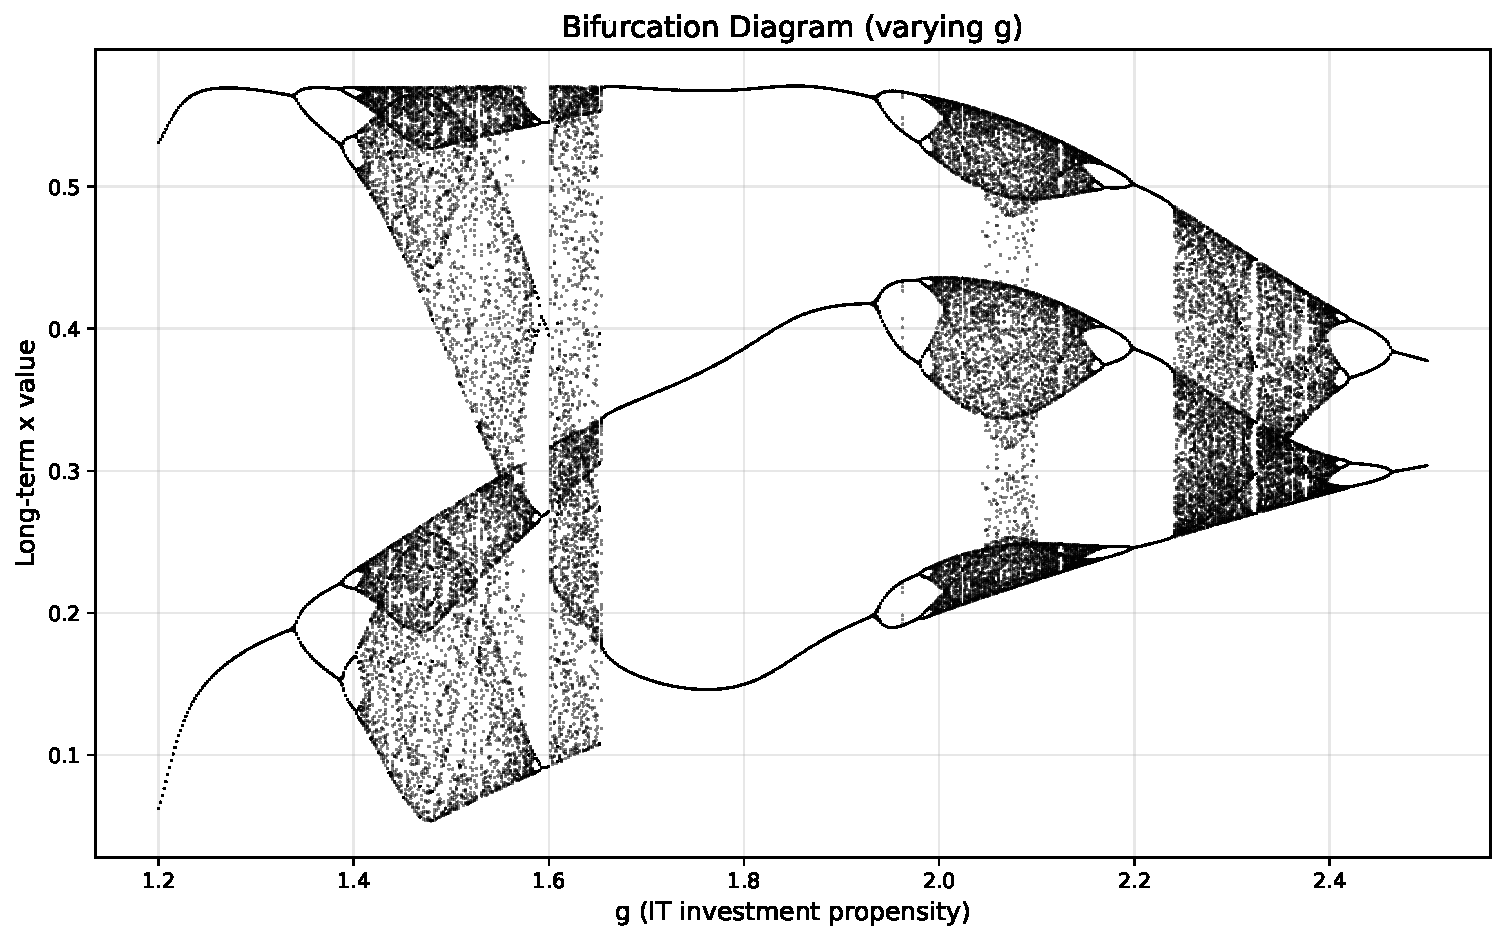
\includegraphics[width=1\textwidth]{../images/results/res-int-3.pdf}
	\caption{Shouldn't this be exposed at Louvre? ($d = 0.5$, $a = 7$, $h = 0.3$, $r = 0.3$, $s = 5.1$)}
	\label{fig:bifurcation}
\end{figure}

\section*{References}
\begin{thebibliography}{9}
	\bibitem{chaos}
	Strogatz, S. H. (2018). \textit{Nonlinear dynamics and chaos: with applications to physics, biology, chemistry, and engineering}. CRC Press.

	\bibitem{italign}
	Luftman, J. (2003). \textit{Assessing IT/business alignment}. Information Systems Management, 20(4), 9-15.

	\bibitem{pyviz}
	Hunter, J. D. (2007). \textit{Matplotlib: A 2D graphics environment}. Computing in science \& engineering, 9(3), 90-95.
\end{thebibliography}

\subsection{Examples}
\appendix
\section{Appendix: Complete Python Code}
The full implementation is available at: \url{https://github.com/Kinshale/pii}

\end{document}
